\documentclass[a4,12pt]{article}
\usepackage{amsmath}
\usepackage{amssymb}
\usepackage[sorting=none]{biblatex}
\usepackage{hyperref}
\usepackage{graphicx}
\usepackage{subcaption}
% limit page margin
\usepackage[margin=1.2in]{geometry}
\usepackage{biblatex}

\addbibresource{{../reference.bib}}
\graphicspath{{../figures/}}
\title{Proposal for PhD Research: 
Quantifying the Uncertainty in both On and Off-target Activity of Prime Editing}
\author{Peiheng Lu}

\begin{document}

\maketitle

Prime editing is a novel gene editing technology that enables theoretically any base substitution, insertion, and deletion without the need for double-strand breaks or donor DNA templates\cite{liudavidr.SearchreplaceGenomeEditing2019,liuPrimeEditingPrecise2023}. Shown in Figure \ref{fig:prime-editing-process}, the prime editors's versatility can mostly be attributed to the reverse transcription mechanism. After the Cas9 nickase cleaves the target DNA strand, the PBS (prime binding site) portion of the pegRNA (prime editing guide RNA) hybridizes with the now floating 3' end of the target DNA strand. The reverse transcriptase (RT) then extends the 3' end of the target DNA strand using the RT template sequence in the pegRNA. The resulting DNA-RNA hybrid is then resolved by the endogenous DNA repair machinery, resulting in the desired edit.

Due to its superior capability, prime editors have the potential to cure up to 90\% of diseases resulted from genetic mutations. However, its clinical application is still limited by the frequently low on target efficiency and the potential off-target activity\cite{zhaoPrimeEditingAdvances2023}.

My master's thesis focused on predicting the on-target activity of prime editing using ensemble learning techniques and the Transformer model to improve pegRNA guide design qualities and thus overall efficiency, and achieved state-of-the-art performance on several existing datasets. As a result, moving on to the prediction of off-target activity of prime editing is a natural next step.

With the recent development of a number of off-target site detection protocols supporting prime editors, it is now more and more possible to quantify their off target activity using big data and deep learning techniques\parencite{liangGenomewideProfilingPrime2023,
zhuTrackingseqRevealsHeterogeneity2024}.
A number of off-target prediction tools have been developed for CRISPR-Cas9, which makes up part of the prime editing system, while DeepPrime-Off developed via fine tuning DeepPrime on the off target sites remains as one of the few prime editing off-target prediction tools. Although the CRISPR-Cas9 system was an essential part of the prime editing system, as studies have pointed out, the reverse transcription process involving the PBS and RT sequences can also impact the off-target activity. Thus, novel tools are needed to produce more accurate predictions the off-target activity of prime editing\parencite{liangGenomewideProfilingPrime2023,yuPredictionEfficienciesDiverse2023}.

On top of extending the model to predict the off-target activity of prime editing, I propose to develop an model capable of outputting the probability distribution of the editing efficiency, rather than a point estimation.

Although majority of the existing solution (including my master's thesis) was aiming at producing a point estimation as the predicted editing efficiency\parencite{mathisMachineLearningPrediction2024,yuPredictionEfficienciesDiverse2023,koeppelPredictionPrimeEditing2023}, the energy-driven binding and cleavage processes are stochastic in nature\cite{stortzPiCRISPRPhysicallyInformed2023}. Thus, it could be more informative to model the posterior distribution of the activity of prime editing given the target loci and pegRNA sequence. An example benefit would be allowing researchers to select the guide design that has smaller variance in editing outcome, if multiple guides showed similar mean editing efficiency.

Recently, a probabilistic deep learning model, crispAI, was proposed to fit a zero inflated negative binomial distribution to the off-target activity of CRISPR-Cas9 on each potential target site\parencite{ozdenLearningQuantifyUncertainty2024}. It was able to accuracy predict the off-target activity in both minimal activity and high activity sites .....

To validate the probabilistic approach, I conducted some preliminary experiments on the on-target prediction of prime editing efficiency using the mathis et al's 90k PE2 HEK293T dataset\parencite{mathisPredictingPrimeEditing2023}. 

(Add details of the experiment and results)

Additional methods including Monte Carlo dropout\parencite{galDropoutBayesianApproximation2016}/Deep ensemble can also be relatively easily applied to gauge the confidence of the model's prediction.


\begin{figure}
    \centering
    \begin{subfigure}{0.4\textwidth}
        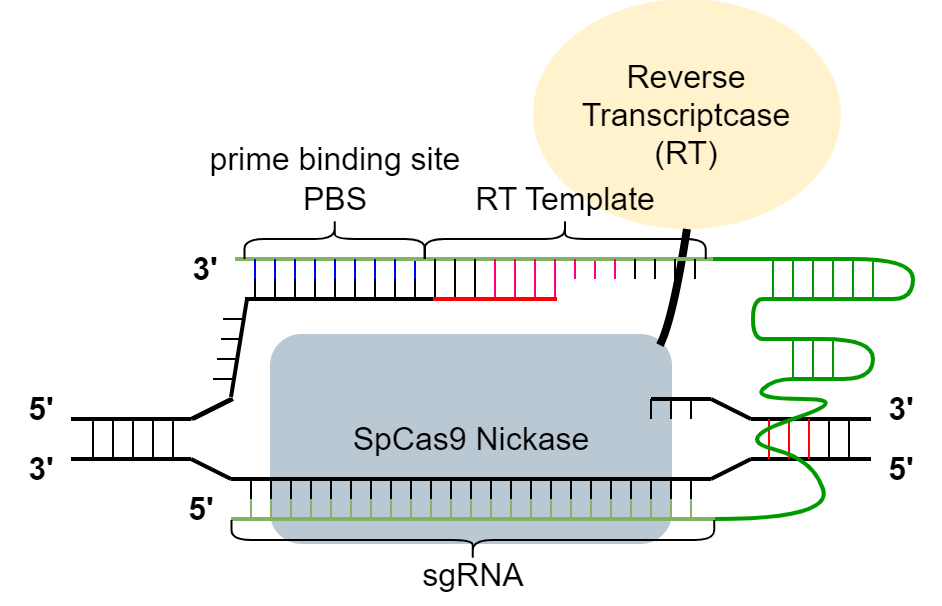
\includegraphics[width=\textwidth]{prime-editing-process.png}
        \caption{Prime editing process}
        \label{fig:prime-editing-process}
    \end{subfigure}
    \begin{subfigure}{0.3\textwidth}
        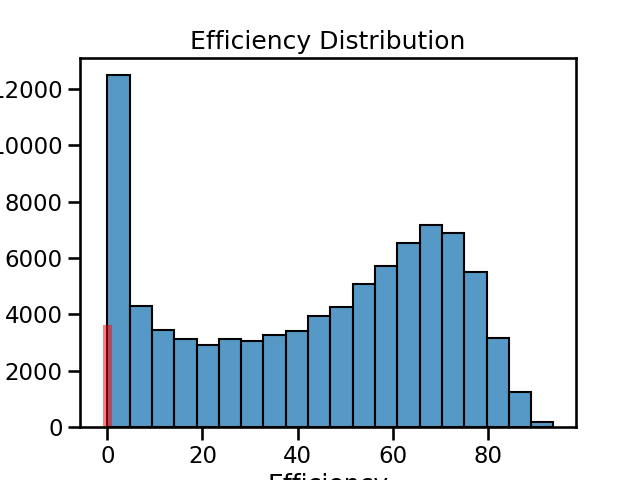
\includegraphics[width=\textwidth]{efficiency_distribution.png}
        \caption{Distribution of measured editing efficiency}
    \end{subfigure}
\end{figure}

Overall, with the on and off target activity of prime editing quantified, we can provide a complete overview of the outcome of using a specific pegRNA sequence on a specific target loci in a specific cell line. This should noticeably improve the safety and efficiency of prime editing, and thus accelerate its clinical application, which would be a long-term goal of my PhD research. 

Last year saw the first FDA approved CRISPR therapy - Casgevy - for the treatment of sickle cell disease, which took a remarkably short time of 11 years to go from the first CRISPR-Cas9 paper to the first FDA approval\cite{CRISPRClinicalTrials}. This is highly inspiring for more advanced CRISPR technologies including base editing and prime editing, both of which have been shown to have great potential in curing genetic diseases. I am planning to make contact with various wet labs to validate the model's prediction on their prime editing experiments, understanding their needs and better incorporating the in silico development model into their workflow. 

\printbibliography

\end{document}